Recently, a few methods have been proposed to address the problem of learning on heterogeneous heterophilic graphs. Some methods used heterogeneous graph neural networks (HGNNs) with mechanism to separate the graph into different subgraphs based on meta-paths and relations edge type \cite{lu2024h2sgnn,guo2023hdhgr,shen2024latgrl}. Other methods used spectral filtering to capture the heterophilic patterns in the graph \cite{lu2024h2sgnn,guo2023hdhgr}. Some are using rewiring techniques to modify the graph structure and improve the learning performance \cite{shen2024latgrl,wang2025hgms}. Some methods used latent-graph construction to learn a latent representation of the graph that captures the heterophilic patterns \cite{shen2024latgrl}. Some methods used contrastive objectives to learn representations that are robust to heterophilic patterns \cite{tao2025cthge}. Some methods used cross-type homophily measurements to capture the heterophilic patterns in the graph \cite{tao2025cthge}. Some also try to preserve heterophiliy by keeps local structure information via sheaf \cite{braithwaite2024hetsheaf}

Many existing methods either focus on heterogeneous graph but not consider heterophily \cite{hu2020heterogeneous,mao2023hinormer,he2024spectral,yang2023simple,wang2019heterogeneous,zhang2019heterogeneous} or focus on heterophilic graph but no consider heterogeneous graph \cite{grover2025spectro, yue2025graph,bodnar2022neural,ribeiro2026cooperative}. Recently, several research have targeted heterogeneous heterophilic graphs and captured heterophily by using several approaches, such as using meta-path-specific spectral filtering \cite{lu2026addressing}, graph rewiring \cite{guo2023homophily,tao2025cross}, unsupervised graph learning \cite{shen2025heterophily,wang2025homophily}, graph transformers \cite{lin2025heterophily}, or learnable mappings \cite{braithwaite2024heterogeneous}.
Other recent approaches explicitly measure or adapt to meta-path-level heterophily through masked prediction objectives \cite{li2025hetero2net} or hop- and meta-path-specific convolution \cite{chen2025adaptive}.
These approaches improve message passing under mixed node and relation types, but they still mainly use typed paths, latent graphs, filters, or edited graphs to determine how node representations are aggregated.
They usually do not preserve a concrete typed path occurrence as a learnable structure that couples its participating edges.
This leaves open how to model higher-order typed relational patterns directly, rather than only using them to define node-level communication channels.

One of the important property of heterogeneous graphs is their ability to capture complex relationships between different node types via meta-paths. Meta-paths are \cite{sun2011pathsim}. Nevertheless, existing methods are not able to capture the higher-order structure of the graph because they neglect meta-paths completely, or use meta-paths mainly to decide which nodes exchange information. They  usually collapse each typed path into a node-to-node view, filter, or edited edge set for message passing \cite{lu2026addressing,chen2025adaptive,li2025hetero2net,guo2023homophily,shen2025heterophily,wang2025homophily}. For instance, a citation network may have relation called co-authorship, where in a graph it is described as a paper--author--paper meta-path, but most research just collapse it to becomes a paper--paper communication channel. 
This preserves endpoint semantics, but it does not explicitly model how the two author--paper edges inside that concrete path jointly interact.  This is useful, but it flattens a concrete path instance into a node-level communication channel. As a result, the model does not explicitly learn how the edges inside the same typed path jointly interact nor how the higher-order relationship of the graph is formed. This motivates modeling selected path instances as higher-order structures over both nodes and edges.



One important property of heterogeneous graphs is meta-path due to  their ability to capture complex relationships between different node types. 
A meta-path defines a typed sequence of relations that describes a composite semantic relation between nodes \cite{sun2011pathsim}. 
Nevertheless, existing methods are still limited in how they use these structures. 
Some methods do not use meta-paths explicitly, while others use them mainly to decide which nodes should exchange information. 
They usually collapse each typed path into a node-to-node view, filter, or edited edge set for message passing \cite{lu2026addressing,chen2025adaptive,li2025hetero2net,guo2023homophily,shen2025heterophily,wang2025homophily}. 
For example, in a citation network, a paper--author--paper meta-path can describe that two papers are connected through a shared author, but most methods convert this pattern into a paper--paper communication channel. 
This preserves the endpoint-level semantic relation, but it does not explicitly model how the two paper--author edges inside that concrete path jointly interact. 
As a result, the model uses the meta-path to guide node aggregation, while the internal edge structure of the path is not directly represented and the representation of the meta-paths themselves are lost, resulting in a loss of higher-order relational information and lower predictive performance.

Another important concern is meta-path selection and searching. Meta-paths are important structure and usually given in advance, but some meta-paths might not be hidden which didn't discovered via human expertise, or even real life datasets might not have meta-paths. Therefore, meta-path discovery is crucial for effectively learning from heterogeneous heterophilic graphs. Some methods use manually specified meta-paths \cite{wang2019han,fu2020magnn}, while others search for meta-paths automatically \cite{yan2024lmsps,jiang2022pmmm}. However, 

Heterogeneous graphs are a common representation for modeling complex relational structures, such as citation 
networks \cite{liu2014meta} or social interactions \cite{singh2025overview}. Unlike homogeneous graphs, heterogeneous graphs contain multiple types of nodes and edges which represents different semantic roles and have different meanings such as citation networks that have authors, papers, and venues node types. \cite{sun2013mining}. Moreover, in recent study, it has been observed that graphs can have property named heterophily, where nodes may have different properties. Therefore, the graph can be heterogeneous heterophilic graphs which has both properties, resulting in a much more complex learning task called heterophilic heterogeneous graphs as shown in Figure \ref{fig:het_hom_graph}. Additionally, modeling graphs under the simplifying assumptions of homogeneity or homophily can obscure important structural and relational patterns. This mismatch provides the model with an incomplete representation of the original graph and may consequently degrade predictive performance \cite{lin2025heterophily}. 

\begin{figure}
  \centering
  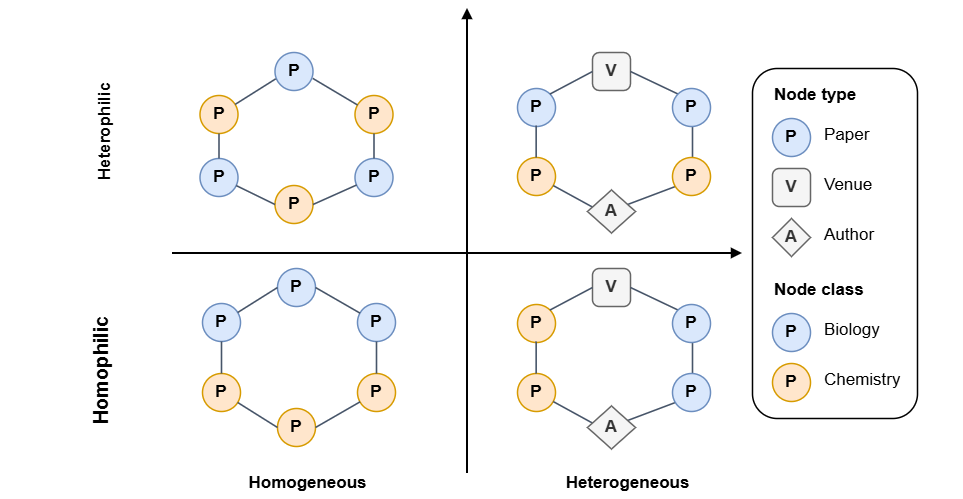
\includegraphics[width=\columnwidth]{figure/Het_HomGraph.drawio.png}
  \caption{An example of heterogeneous heterophilic graph. The graph contains multiple types of nodes and edges, and connected nodes may have different properties.}
  \Description{An example of heterogeneous heterophilic graph. The graph contains multiple types of nodes and edges, and connected nodes may have different properties.}
  \label{fig:het_hom_graph}
\end{figure}

Many existing methods either focus on heterogeneous graph but not consider heterophily \cite{hu2020heterogeneous,mao2023hinormer,he2024spectral,yang2023simple,wang2019heterogeneous,zhang2019heterogeneous} or focus on heterophilic graph but no consider heterogeneous graph \cite{grover2025spectro, yue2025graph,bodnar2022neural,ribeiro2026cooperative}. Recently, several research have targeted heterogeneous heterophilic graphs and captured heterophily by using several approaches, such as using meta-path to construct latent subgraphs suitable for learning heterophily and heterogeneity \cite{lu2026addressing,chen2025adaptive,li2025hetero2net,guo2023homophily,shen2025heterophily,wang2025homophily}, graph rewiring across node types \cite{tao2025cross}, using transformer directly in heterogeneous graphs \cite{lin2025heterophily}, or learnable mappings in heterogeneous graphs \cite{braithwaite2024heterogeneous}. 

One important property of heterogeneous graphs is meta-path due to  their ability to capture complex relationships between different node types. 
A meta-path defines a typed sequence of relations that describes a composite semantic relation between nodes \cite{sun2011pathsim}. 
Nevertheless, existing methods are still limited in how they use these structures. 
Some methods do not use meta-paths explicitly, while others use them mainly to decide which nodes should exchange information. 
They usually collapse each typed path into a node-to-node view, filter, or edited edge set for message passing \cite{lu2026addressing,chen2025adaptive,li2025hetero2net,guo2023homophily,shen2025heterophily,wang2025homophily}. 
For example, in a citation network, a paper--author--paper meta-path can describe that two papers are connected through a shared author, but most methods convert this pattern into a paper--paper communication channel. 
This preserves the endpoint-level semantic relation, but it does not explicitly model how the two paper--author edges inside that concrete path jointly interact. 
As a result, the model uses the meta-path to guide node aggregation, while the internal edge structure of the path is not directly represented and the representation of the meta-paths themselves are lost, resulting in a loss of higher-order relational information and lower predictive performance.

\documentclass[sigconf,anonymous,review]{acmart}

\usepackage{amsthm}
\usepackage{algorithm}
\usepackage{algorithmic}

\AtBeginDocument{%
  \providecommand\BibTeX{{Bib\TeX}}}

% Replace the ACM metadata below with the values supplied by the proceedings venue.
\setcopyright{acmlicensed}
\copyrightyear{2026}
\acmYear{2026}
\acmDOI{XXXXXXX.XXXXXXX}
\acmConference[Conference acronym 'XX]{ACM Conference}{Month DD--DD, 2026}{City, Country}
\acmISBN{978-1-4503-XXXX-X/2026/MM}

\newcommand{\R}{\mathbb{R}}
\newcommand{\method}{\textsc{H2S-NN}}
\newcommand{\ampss}{\textsc{AMPSS}}
\newcommand{\thspool}{\textsc{THS-Pool}}
\newcommand{\cF}{\mathcal{F}}
\newcommand{\cL}{\mathcal{L}}
\newcommand{\norm}[1]{\left\lVert #1\right\rVert}
\newcommand{\transpose}{\mathsf{T}}
\newcommand{\concat}{\mathbin\Vert}
\newtheorem{proposition}{Proposition}

\title[H2S-NN]{H2S-NN: Heterogeneous Sheaf--Hodge Neural Networks with Adaptive Schema-to-Cell Selection}

% Replace the affiliation placeholder before submission.
\author{Peeradon Sarnkaew}
\email{peeradonsarnkaew46@gmail.com}
\affiliation{%
  \institution{Independent Researcher}
  \city{Bangkok}
  \country{Thailand}
}
\renewcommand{\shortauthors}{Sarnkaew}

\begin{document}

\begin{abstract}
Heterogeneous graphs combine several node and relation types, while many of their observed
relations are heterophilic. Conventional heterogeneous graph neural networks represent typed
paths as message-passing channels, and existing heterogeneous sheaf networks learn a geometry on
the observed graph but remain confined to its nodes and edges. We introduce \method, a
heterogeneous sheaf--Hodge architecture in which concrete typed path instances provide
higher-order, face-like supports for diffusion over an explicit edge cochain. Relation-conditioned
node-to-edge maps define a learned first coboundary, an ordered sequence encoder constructs
edge-to-face maps, and matrix-free lower and upper Hodge terms evolve node and edge states without
materializing global block matrices. We further introduce \ampss, a two-stage selection procedure
that enumerates typed schemas, ranks them using training-only task signals and structural coverage,
and refines the retained schemas and instances through differentiable nonnegative gates inside the
upper edge Laplacian. We state precisely where the current construction differs from a strict
cellular cochain complex: synthetic closure pairs correct the node Laplacian, whereas the learned
second coboundary remains path-edge-only and $\delta_1\delta_0=0$ is encouraged rather than
guaranteed. Across the completed evaluation, \method{} obtains the strongest reported average in
all six node-classification columns and all eight node-clustering columns; it ties the MUTAG
ceiling and leads the remaining graph-classification comparisons. On link prediction it leads
both measures on LastFM and AUPR on PubMed, while remaining competitive on Amazon and YouTube.
On ACM it also records the lowest runtime, parameter count, and peak memory among the compared
systems. A DBLP ablation attributes additional gains to automatic schema selection and
instance-level refinement. The in-development \thspool{} hierarchical graph-pooling extension is
intentionally reserved as a placeholder and is not used to support these claims.
\end{abstract}

\ccsdesc[500]{Computing methodologies~Neural networks}
\ccsdesc[300]{Mathematics of computing~Graph theory}
\ccsdesc[300]{Information systems~Data mining}

\keywords{heterogeneous graph neural networks, sheaf neural networks, Hodge Laplacian, meta-path discovery, heterophily}

\maketitle

\section{Introduction}
\label{sec:introduction}


Heterogeneous graphs are a common representation for modeling complex relational structures, such as citation 
networks \cite{liu2014meta} or social interactions \cite{singh2025overview}. Unlike homogeneous graphs, heterogeneous graphs contain multiple types of nodes and edges which represents different semantic roles and have different meanings such as citation networks that have authors, papers, and venues node types. \cite{sun2013mining}. Moreover, in recent study, it has been observed that graphs can have property named heterophily, where nodes may have different properties. Therefore, the graph can be heterogeneous heterophilic graphs which has both properties, resulting in a much more complex learning task called heterophilic heterogeneous graphs as shown in Figure \ref{fig:het_hom_graph}. Additionally, modeling graphs under the simplifying assumptions of homogeneity or homophily can obscure important structural and relational patterns. This mismatch provides the model with an incomplete representation of the original graph and may consequently degrade predictive performance \cite{lin2025heterophily}. 

\begin{figure}
  \centering
  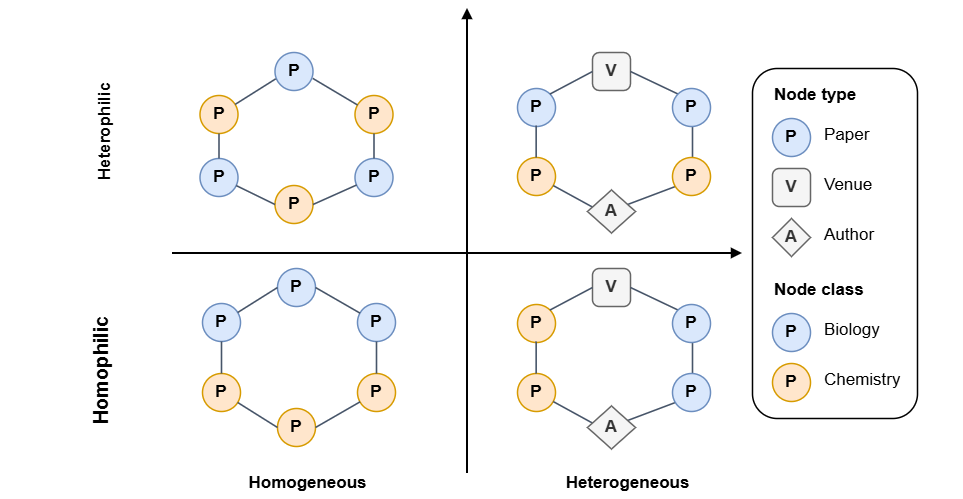
\includegraphics[width=\columnwidth]{figure/Het_HomGraph.drawio.png}
  \caption{An example of heterogeneous heterophilic graph. The graph contains multiple types of nodes and edges, and connected nodes may have different properties.}
  \Description{An example of heterogeneous heterophilic graph. The graph contains multiple types of nodes and edges, and connected nodes may have different properties.}
  \label{fig:het_hom_graph}
\end{figure}

Many existing methods either focus on heterogeneous graph but not consider heterophily \cite{hu2020heterogeneous,mao2023hinormer,he2024spectral,yang2023simple,wang2019heterogeneous,zhang2019heterogeneous} or focus on heterophilic graph but no consider heterogeneous graph \cite{grover2025spectro, yue2025graph,bodnar2022neural,ribeiro2026cooperative}. Recently, several research have targeted heterogeneous heterophilic graphs and captured heterophily by using several approaches, such as using meta-path to construct latent subgraphs suitable for learning heterophily and heterogeneity \cite{lu2026addressing,chen2025adaptive,li2025hetero2net,guo2023homophily,shen2025heterophily,wang2025homophily}, graph rewiring across node types \cite{tao2025cross,}, using transformer directly in heterogeneous graphs \cite{lin2025heterophily}, or learnable mappings in heterogeneous graphs \cite{braithwaite2024heterogeneous}. 

Moreover, meta-paths provide a natural way to describe composite relations in heterogeneous graphs. A
meta-path is a typed sequence of relations, such as paper--author--paper, that connects two papers
through a shared author and therefore expresses information that is not contained in either
endpoint alone \cite{sun2011pathsim}. Existing heterophilic heterogeneous graph neural networks use meta-path sequences to construct
a node-to-node view, filter, or edited edge set for message passing
\cite{lu2026addressing,chen2025adaptive,li2025hetero2net,guo2023homophily,shen2025heterophily,wang2025homophily}.
This treatment preserves the composite relation between the endpoints, but the concrete path
instance is no longer represented after the induced neighbourhood has been formed. In the example
above, the path determines which papers may exchange information, while the two paper--author
relations inside that path do not remain as a joint structure that can directly shape propagation.

Furthermore, meta-paths are usually given in advance, but some meta-paths might not be hidden which didn't discovered via human expertise, or even real life datasets might not have meta-paths. Therefore, meta-path discovery is crucial for effectively learning from heterogeneous heterophilic graphs. Some methods use manually specified meta-paths \cite{wang2019han,fu2020magnn}, while others search for meta-paths automatically \cite{yan2024lmsps,jiang2022pmmm}. However, these methods still mainly use typed paths to define node-level communication channels rather than retaining them as higher-order structures that directly shape diffusion over both nodes and edges.

Therefore, This limitation motivates the central question of this work: can a heterogeneous graph model
learn not only how signals propagate, but also which higher-order relational structures should
support that propagation and, for graph-level tasks, how the resulting geometry should be
summarized across resolutions? We address this question with \method{}, a unified heterogeneous
sheaf--Hodge framework with three connected components. Its fine-scale backbone turns meta-path instances into operator-level with graph message passing by designing graph as 2D-complex. \ampss{} determines which schemas
and instances populate those supports; and \thspool{} preserves the learned node-level sheaf
geometry while constructing hierarchical representations for graph classification.



At the fine resolution, \method{} changes the role of a typed path from an aggregation route to an
input of the diffusion operator. Relation-conditioned node-to-edge maps define a learned first
coboundary, while an ordered sequence encoder constructs edge-to-face maps for the selected path
instances. The resulting lower and upper Hodge terms evolve an explicit edge cochain alongside the
node cochain, so a selected path can couple its participating edges through the upper edge
Laplacian. We use ``face-like'' deliberately: the learned second coboundary remains path-edge-only,
and the exact chain condition $\delta_1\delta_0=0$ is encouraged by the objective rather than
guaranteed by construction.

Graph-level prediction raises a complementary problem. A flat terminal readout summarizes the
fine representation but does not explicitly model its organization across resolutions, whereas an
arbitrary graph reduction can distort the geometry learned by the sheaf operator. We therefore
introduce \thspool{} (Typed Hierarchical Sheaf Pooling via Galerkin coarsening) as the graph-level
branch of \method{}. \thspool{} learns type-aware assignments from fine nodes to typed coarse
entities and uses the induced prolongation $P_0$ to define the coarse node operator
$L_{0,c}=P_0^{\transpose}L_0P_0$. Consequently, every coarse cochain $z$ satisfies
$z^{\transpose}L_{0,c}z=(P_0z)^{\transpose}L_0(P_0z)$, so coarse diffusion measures exactly the
fine-scale node-sheaf energy of the lifted signal. The implemented Galerkin stage coarsens $L_0$;
it does not yet claim a corresponding coarsening of the edge operator $L_1$. Node classification,
node clustering, and link prediction instead use their task-specific readouts without hierarchical
coarsening.

Together, the three components address a common objective at different stages of the pipeline:
\ampss{} selects the typed higher-order support, the sheaf--Hodge backbone learns diffusion over node
and edge ranks, and \thspool{} constructs an energy-consistent hierarchy when a graph-level
prediction is required.

The contributions of this work are as follows.
\begin{enumerate}
  \item We introduce \method{}, a heterogeneous sheaf--Hodge framework that retains concrete typed
  path instances as face-like, operator-level supports. Relation-conditioned node-to-edge maps,
  sequence-conditioned edge-to-face maps, and matrix-free Hodge terms jointly evolve node and edge
  cochains without materializing global block matrices.
  \item We propose \ampss{}, a two-stage schema-to-cell selection mechanism that combines
  training-only candidate preselection with differentiable schema- and instance-level refinement
  inside the upper edge Laplacian.
  \item For graph classification, we introduce \thspool{}, which learns type-aware coarse
  assignments and applies Galerkin coarsening to the learned node-sheaf operator. Its construction
  preserves the fine-scale quadratic energy of every lifted coarse signal by design.
  \item We analyze the framework's scope and operator properties, including the positivity of its
  weighted Hodge terms, the Galerkin energy identity, and the lack of a guaranteed exact chain
  condition in the path-supported construction.
  \item We evaluate the framework across node classification, graph classification, node
  clustering, and heterogeneous link prediction, with controlled studies of automatic
  schema-to-cell selection, typed Galerkin coarsening, and computational cost.
\end{enumerate}


\section{Background and Related Work}
\label{sec:background}
\subsection{Heterogeneous heterophily learning}

Recent work has begun to study graphs that are both heterogeneous and heterophilic. 
One line measures heterophily through meta-path or cross-type homophily statistics. 
Hetero$^2$Net identifies heterophily in heterogeneous graphs using meta-path-based metrics and introduces masked meta-path and masked label prediction objectives \cite{li2023hetero2net}. 
HDHGR defines a meta-path-induced homophily measure and uses it to guide heterogeneous graph rewiring \cite{guo2023hdhgr}. 
CTHGE introduces a cross-type homophily ratio and edits cross-type connectivity according to this measurement \cite{tao2025cthge}.

A second line designs heterophily-aware propagation or filtering mechanisms. 
H2SGNN decomposes the graph into meta-path-induced subgraphs and applies local independent spectral filters, while using a global hybrid filter to capture higher-order neighbours \cite{lu2024h2sgnn}. 
AHGNN learns hop- and meta-path-specific adaptive convolution and combines semantic information through coarse-to-fine fusion \cite{chen2025ahgnn}. 
H2G-Former, introduced with the H2GB benchmark, combines masked label embeddings, cross-type heterogeneous attention, and type-specific feed-forward networks for heterogeneous heterophilic graph learning \cite{lin2024h2gb}.

A third line modifies the graph representation or training objective. 
LatGRL constructs homophilic and heterophilic latent graphs from coupled structural and attribute similarity, then fuses semantic signals through an adaptive dual-frequency mechanism \cite{shen2024latgrl}. 
HGMS performs heterogeneous graph contrastive learning with connection-strength-guided edge retention and multi-view self-expression \cite{wang2025hgms}. 
HetSheaf learns type-aware sheaf restriction maps on heterogeneous graphs, replacing direct feature averaging with learned transport over the observed node-edge structure \cite{braithwaite2024hetsheaf}.

These methods are important baselines because they directly address the interaction between heterogeneity and heterophily. 
However, their mechanisms mainly improve node-level representation learning through meta-path views, spectral filters, rewiring, latent graphs, contrastive augmentation, or learned node-edge transport. 
They do not keep each concrete typed path occurrence as an explicit edge-coupling structure that directly changes the diffusion operator. 
This distinction motivates \method{}, which uses selected typed path instances to shape diffusion over both node and edge states.

\subsection{Heterogeneous graphs and typed paths}

A heterogeneous graph is a tuple $G=(V,E,\phi,\psi)$, where $\phi:V\rightarrow\mathcal{T}$ and
$\psi:E\rightarrow\mathcal{R}$ assign node and relation types. A meta-path schema
$\sigma=(t_0,r_1,t_1,\ldots,r_\ell,t_\ell)$ specifies a valid walk in the type graph. A concrete
instance $f=(v_0,e_1,v_1,\ldots,e_\ell,v_\ell)$ follows that schema in $G$. HAN and MAGNN aggregate
features over manually specified meta-path views \cite{wang2019han,fu2020magnn}, whereas HGT uses
typed attention without requiring explicit paths \cite{hu2020hgt}. LMSPS progressively searches
long-range paths, and PMMM searches a differentiable meta-multigraph while using partial message
propagation to improve stability \cite{yan2024lmsps,jiang2022pmmm}. These methods search or weight
communication structures; they do not retain each path instance as an element of a second
coboundary operator.

\subsection{Cellular sheaves and neural diffusion}

A cellular sheaf $\cF$ on a graph assigns a vector space $\cF(v)$ to each node, a vector space
$\cF(e)$ to each edge, and a linear restriction map $F_{v\unlhd e}:\cF(v)\rightarrow\cF(e)$ for
each incident pair. With a chosen edge orientation, the first coboundary compares transported
endpoint signals,
\begin{equation}
  (\delta_0 x)_e = F_{t(e)\unlhd e}x_{t(e)}-F_{s(e)\unlhd e}x_{s(e)}.
  \label{eq:background-delta0}
\end{equation}
The associated sheaf Laplacian is $L_0=\delta_0^{\transpose}\delta_0$. When all stalks are
one-dimensional and all restrictions are identities, this reduces to the ordinary graph
Laplacian. Neural Sheaf Diffusion learns the restrictions from data and uses the induced geometry
to control diffusion in heterophilic settings \cite{bodnar2022neural}. HetSheaf conditions the
predictor on node and edge types and develops a gauge-aware graph readout
\cite{braithwaite2024hetsheaf}. \method{} retains typed restriction learning while adding an
explicit edge cochain and a path-supported second operator.

\subsection{Heterophily-aware heterogeneous learning}

Recent methods address heterogeneous heterophily by rewiring, spectral filtering, latent-graph
construction, contrastive objectives, or cross-type homophily measurements
\cite{guo2023hdhgr,lu2024h2sgnn,shen2024latgrl,wang2025hgms,tao2025cthge}. These approaches are
important baselines because they target the same failure mode of naive neighbour averaging. Their
mechanism is nevertheless different from learning maps on node--edge and edge--face incidences.

\subsection{Positioning}

Table~\ref{tab:positioning} summarizes the boundary of the contribution. We use ``face-like''
deliberately: Section~\ref{sec:closure} explains why the implemented operators form a generalized
path-supported cochain system rather than an exact cellular cochain complex.

\begin{table*}[t]
  \centering
  \caption{Position of \method{} relative to adjacent model families.}
  \label{tab:positioning}
  \small
  \begin{tabular}{p{0.16\textwidth}p{0.38\textwidth}p{0.38\textwidth}}
    \toprule
    \textbf{Family} & \textbf{Primary mechanism} & \textbf{Difference in \method{}} \\
    \midrule
    HAN / MAGNN & Meta-path views route and aggregate messages. & Concrete path instances remain in an edge-to-face operator. \\
    HGT & Typed attention over the observed graph. & Adds an explicit edge cochain and a learned upper edge term. \\
    LMSPS / PMMM & Automatically select schemas or meta-multigraph channels. & Selected structures weight $\delta_1^{\transpose}\delta_1$, not only aggregation. \\
    Neural Sheaf Diffusion & Learned sheaf diffusion on a homogeneous 1-skeleton. & Conditions on heterogeneous types and introduces path-supported edge diffusion. \\
    HetSheaf & Heterogeneous restriction maps and gauge-aware readout. & Adds ordered edge-to-face maps and an explicit edge Hodge operator. \\
    \bottomrule
  \end{tabular}
\end{table*}

\subsection{Related Works}
Several methods have begun to study heterogeneous heterophilic graphs directly. 
Hetero$^2$Net identifies heterophily in heterogeneous graphs using meta-path-based measurements and introduces masked meta-path and masked label prediction objectives \cite{li2023hetero2net}. 
H2SGNN decomposes the graph into meta-path-induced subgraphs and applies local independent spectral filters, together with a global hybrid filter for higher-order neighbors \cite{lu2024h2sgnn}. 
HDHGR measures meta-path-induced homophily and rewires heterogeneous graphs to improve homophily-oriented message passing \cite{guo2023hdhgr}. 
LatGRL constructs homophilic and heterophilic latent graphs by coupling structural and attribute similarity, then fuses semantic information with an adaptive dual-frequency mechanism \cite{shen2024latgrl}. 
HGMS uses heterogeneous graph contrastive learning with connection-strength-guided edge retention and multi-view self-expression \cite{wang2025hgms}. 
CTHGE introduces a cross-type homophily ratio and edits cross-type graph connectivity according to this measurement \cite{tao2025cthge}. 
AHGNN further learns hop- and meta-path-specific adaptive convolution with coarse-to-fine semantic fusion \cite{chen2025ahgnn}, while H2G-Former is introduced with the H2GB benchmark to evaluate graph learning under both heterophily and heterogeneity \cite{lin2024h2gb}. 
HetSheaf extends sheaf neural networks to heterogeneous graphs by learning type-aware restriction maps on the observed node-edge structure \cite{braithwaite2024hetsheaf}.
Although these methods improve learning under heterogeneous heterophily, they mainly use meta-paths, latent graphs, spectral filters, contrastive views, or graph edits to improve node-level message passing. 
They do not explicitly keep each concrete typed path occurrence as a structure that couples the participating edges and directly changes the diffusion operator.
\section{H2S-NN}
\label{sec:method}

\subsection{Problem setting and notation}

Let $N=|V|$ and $M=|E|$. We use a common stalk dimension $d$ for node, edge, and
face-output vectors, a relation-embedding dimension $d_r$, and a sequence hidden dimension $d_h$.
Node and edge cochains are $x\in\R^{N\times d}$ and $s\in\R^{M\times d}$. The $F$ selected path
instances contain $I=\sum_{f=1}^{F}|\partial f|$ path-edge incidences. Superscripts ``src'' and
``tgt'' denote the two node-to-edge restriction maps of an oriented edge;
$A_{e\triangleright f}$ denotes an edge-to-face map. Adjoint operators are written with
$\transpose$ because the implementation uses the Euclidean inner product on every stalk.

\begin{figure*}[t]
  \centering
  \setlength{\fboxsep}{6pt}
  \begin{tabular}{@{}c@{\hspace{0.5em}}c@{\hspace{0.5em}}c@{\hspace{0.5em}}c@{}}
    \fbox{\parbox{0.20\textwidth}{\centering\textbf{1. Typed input}\\pad features; encode node and relation types}} &
    \fbox{\parbox{0.20\textwidth}{\centering\textbf{2. Path support}\\manual schemas or \ampss; enumerate instances}} &
    \fbox{\parbox{0.20\textwidth}{\centering\textbf{3. Geometry}\\learn node--edge and edge--face maps}} &
    \fbox{\parbox{0.20\textwidth}{\centering\textbf{4. Prediction}\\Hodge diffusion; task readout}}
  \end{tabular}
  \caption{The \method{} pipeline. Selected path instances act through learned edge-to-face maps
  and the upper component of the edge operator.}
  \Description{A four-stage pipeline from typed graph input, to selected path supports, learned geometry, and final prediction.}
  \label{fig:pipeline}
\end{figure*}

\subsection{Typed input representation}

Raw feature matrices may have different widths across node types. The data layer pads them to a
common width and appends relation-level structural statistics derived using training labels only.
For a node $v$ of type $\phi(v)$, the implemented encoder is
\begin{equation}
  h_v^{(0)}=\operatorname{Dropout}\!\left(
  \operatorname{GELU}\!\left(
  \operatorname{LN}\!\left(W_{\phi(v)}x_v+b_{\phi(v)}\right)+q_{\phi(v)}
  \right)\right)\in\R^d,
  \label{eq:node-encoder}
\end{equation}
where each node type has a separate affine map and $q_t$ is a learned type embedding. If a graph
has no node features, a free embedding table supplies one learned $d$-vector per node; this avoids
the bias-only collapse of a zero-width linear layer. Each relation $r$ has an embedding
$z_r\in\R^{d_r}$.

\subsection{Relation-conditioned node-to-edge maps}

For every stored directed edge $e=(u\xrightarrow{r}v)$, two relation-specific MLPs receive
$[h_u^{(0)}\concat h_v^{(0)}\concat z_r]$ and predict maps
$F_e^{\mathrm{src}},F_e^{\mathrm{tgt}}\in\R^{d\times d}$. The default maps are conformal,
\begin{equation}
  F_e=\lambda_e Q_e,\qquad Q_e^{\transpose}Q_e=I,\qquad
  \lambda_e=\exp(\min\{a_e,2\}),
  \label{eq:conformal-map}
\end{equation}
with $Q_e$ produced by a pure-PyTorch Householder parameterization. Cayley maps are also
implemented, while Euler rotations are restricted to $d\in\{2,3\}$. A matrix-exponential option
is rejected during configuration validation because its full-edge CUDA backward path was unsafe in
the target environment. We call the maps \emph{scaled orthogonal}, not orthogonal.

The learned first coboundary is
\begin{equation}
  (\delta_0 h^{(0)})_e=F_e^{\mathrm{tgt}}h_v^{(0)}-
  F_e^{\mathrm{src}}h_u^{(0)}.
  \label{eq:delta0}
\end{equation}
It is used as an edge feature, but not as the initial edge signal itself.

\subsection{Independent edge-cochain initialization}

The edge initializer preserves information that would be lost by forcing every initial edge state
to be exact:
\begin{equation}
  s_e^{(0)}=\operatorname{MLP}_{\mathrm{init}}\!\left(
  h_u^{(0)}\concat h_v^{(0)}\concat z_r\concat(\delta_0h^{(0)})_e
  \right).
  \label{eq:edge-init}
\end{equation}
The final block is optional through \texttt{use\_delta0\_init}. Initializing
$s^{(0)}=\delta_0h^{(0)}$ would restrict the edge signal to the image of $\delta_0$ and remove an
independent component before diffusion begins.

\subsection{Typed path instances and edge-to-face maps}

In manual mode, dataset-specific templates determine which paths are enumerated. In automatic
mode, Section~\ref{sec:ampss} constructs a fixed candidate pool. For a concrete path instance
$f=(v_0,e_1,v_1,\ldots,e_\ell,v_\ell)$, the sequence module forms tokens
\begin{equation}
  g_i=\operatorname{MLP}_{g}\!
  \left(h_{v_{i-1}}^{(0)}\concat h_{v_i}^{(0)}\concat z_{\psi(e_i)}\right),
  \qquad (o_1,\ldots,o_\ell)=\operatorname{LSTM}(g_1,\ldots,g_\ell).
\end{equation}
A learned vector $a$ gives position attention
\begin{equation}
  \pi_{fi}=\operatorname{softmax}_{i}\left(\frac{o_i^{\transpose}a}{\sqrt{d_h}}\right),
  \qquad
  A_{e_i\triangleright f}=\pi_{fi}\operatorname{reshape}(W_Ao_i+b_A,d,d).
  \label{eq:face-map}
\end{equation}
The attention weight multiplies the map itself. Maps are produced in bounded face chunks, cached
once per forward pass, and reused for all diffusion steps.

\subsection{Closure convention and the chain-condition caveat}
\label{sec:closure}

Every open path has an endpoint pair $(v_\ell,v_0)$ recorded as a synthetic closure edge. The
implementation does not add a stateful closure edge to $s$ and does not include that edge in
$\delta_1$. Instead, it adds the closed-form contribution of a frozen $\gamma I_d$ restriction to
the node Laplacian,
\begin{align}
  C_{\mathrm{cl}}(x)_{v_\ell} &\mathrel{+}=\gamma^2(x_{v_\ell}-x_{v_0}), &
  C_{\mathrm{cl}}(x)_{v_0} &\mathrel{-}=\gamma^2(x_{v_\ell}-x_{v_0}),
  \label{eq:closure}
\end{align}
for every recorded closure occurrence. The default $\gamma=10^{-6}$ yields an effective
$10^{-12}$ coupling.

Because the second operator sees only the stored path edges, independently learned restrictions do
not guarantee $\delta_1\delta_0=0$. We therefore describe the implementation as a generalized,
path-supported sheaf--Hodge system and penalize the composition during training. A future strict
cellular version would materialize a compatible closed boundary and enforce the chain condition by
construction.

\subsection{Matrix-free coboundaries and Hodge operators}

Let $\eta(e,f)\in\{-1,+1\}$ be the stored incidence sign. The second operator is
\begin{equation}
  (\delta_1s)_f=\sum_{e\in\partial_{\mathrm{path}} f}
  \eta(e,f)A_{e\triangleright f}s_e.
  \label{eq:delta1}
\end{equation}
The code supports arbitrary signs and tests a negative-incidence case. Production enumeration
follows stored forward relations, so it currently emits $+1$ for every incidence. The node and
edge operators are
\begin{align}
  L_0x &= \delta_0^{\transpose}\delta_0x+C_{\mathrm{cl}}(x),
  \label{eq:l0}\\
  L_1s &= \underbrace{\delta_0\delta_0^{\transpose}s}_{L_1^{\mathrm{down}}s}
         +\underbrace{\delta_1^{\transpose}\delta_1s}_{L_1^{\mathrm{up}}s}.
  \label{eq:l1}
\end{align}
No global $Nd\times Nd$ or $Md\times Md$ matrix is formed. Batched matrix--vector products and
scatter-add operations implement each operator and its adjoint.

\subsection{Hodge diffusion}

The model performs $K$ explicit Euler steps,
\begin{equation}
  x^{(k+1)}=x^{(k)}-\eta_0L_0x^{(k)},\qquad
  s^{(k+1)}=s^{(k)}-\eta_1L_1s^{(k)},\quad k=0,\ldots,K-1.
  \label{eq:diffusion}
\end{equation}
Learnable step sizes are softplus-parameterized and therefore positive. Optional layer dropout is
applied to both ranks after each step. Layer normalization produces $x^\star$ and $s^\star$.

The ranks are evolved in parallel under operators inferred from the same initial node state; the
implemented recurrence does not feed $s^{(k)}$ into the node update or $x^{(k)}$ into the edge
update. Higher-order information therefore reaches a task only if its readout consumes $s^\star$
or a descriptor derived from it. This observation is central to Section~\ref{sec:experiments}.

\subsection{Task readouts}
\label{sec:readouts}

\paragraph{Node classification.}
Each node receives the mean of its incident edge states,
$\bar{s}_v=|E(v)|^{-1}\sum_{e\ni v}s_e^\star$. Target-type logits are
\begin{equation}
  \widehat{y}_v=\operatorname{MLP}_{\mathrm{node}}
  (x_v^\star\concat h_v^{(0)}\concat\bar{s}_v).
  \label{eq:node-readout}
\end{equation}
This is the present readout through which the face pathway directly affects supervised predictions.

\paragraph{Link prediction.}
The implemented dot, DistMult, and concatenation-MLP decoders score pairs using $x^\star$.
DistMult uses one relation matrix per pooled target relation. Since these decoders do not consume
$s^\star$, the current link-prediction task loss does not directly supervise the upper edge
operator; link experiments validate the shared encoder and data protocol, not the central
higher-order readout claim.

\paragraph{Graph classification.}
The graph-level interface supports mean pooling of $x^\star$ and terminal heads that inspect
$x^\star$, $h^{(0)}$, and incident-edge descriptors derived from $s^\star$. The completed graph
comparison evaluates this terminal-readout setting. The planned hierarchical \thspool{} method is
a separate extension and is not part of that result.

\subsection{Training objective}

For single-label tasks, $\cL_{\mathrm{task}}$ is cross-entropy; IMDB uses multi-label binary
cross-entropy with logits. Link prediction uses binary cross-entropy. Four geometric terms are
shared across trainers:
\begin{align}
  \cL_{0} &= \lambda_0\operatorname{mean}\norm{\delta_0x^\star}_2^2, &
  \cL_{1} &= \lambda_1\operatorname{mean}\norm{\delta_1s^\star}_2^2,\\
  \cL_{\mathrm{cons}} &= \lambda_c\operatorname{mean}\norm{s^\star-\delta_0x^\star}_2^2, &
  \cL_{\mathrm{chain}} &= \lambda_{co}\operatorname{mean}
  \norm{\delta_1\delta_0h^{(0)}}_2^2.
  \label{eq:regularizers}
\end{align}
The last term is a soft chain-consistency penalty, not a proof that the learned maps form an exact
complex. The complete loss is
\begin{equation}
  \cL=\cL_{\mathrm{task}}+\cL_0+\cL_1+\cL_{\mathrm{cons}}+
  \cL_{\mathrm{chain}}+\rho(t)\cL_{\mathrm{disc}},
  \label{eq:loss}
\end{equation}
where $\rho(t)$ is zero during discovery warm-up and optionally increases linearly afterward.

\section{Adaptive Schema-to-Cell Selection}
\label{sec:ampss}

\subsection{Candidate generation and statistics}

\ampss{} begins with a directed type graph whose arcs are the stored relation tuples. Bounded
depth-first search enumerates schemas of length $\ell\in[\ell_{\min},\ell_{\max}]$, optionally
requiring the target type at both ends and allowing repeated types. Candidate count, instances per
anchor, instances per schema, and total materialized instances are separately capped. This is a
preprocessing operation and is non-differentiable.

For node classification, labels on the training mask are propagated for a fixed number of steps to
give distributions $\widehat{y}_v$. A sampled instance receives
\begin{equation}
  d(f)=\norm{\widehat{y}_{v_0}-\widehat{y}_{v_\ell}}_2^2,\qquad
  D(\sigma)=\frac{1}{|\mathcal{I}_\sigma|}\sum_{f\in\mathcal{I}_\sigma}d(f).
  \label{eq:discrepancy}
\end{equation}
Only training labels contribute to $\widehat{y}$. Link prediction uses an analogous two-channel
role signal constructed from training-positive source and target endpoints. Validation and test
positives are excluded. For graph classification, the pool is learned from training graphs only:
schema presence is counted by class and scored by the variance of class-normalized occurrence,
with a small log-frequency tie breaker. This graph-level score is task-specific and should not be
conflated with Equation~\ref{eq:discrepancy}.

The node/link path also records instance count, start and end coverage, relation diversity, type
diversity, average branching, estimated cost, and sampled endpoint sets. The structural instance
feature tensor is stored for analysis but is not currently an input to $\beta_f$.

\subsection{Greedy pool and differentiable refinement}

For node and link tasks, if $S$ is the set already selected, the score is
\begin{equation}
  q(\sigma\mid S)=
  \frac{D(\sigma)^{a_d}\,C(\sigma)^{a_c}\,V(\sigma)^{a_v}}
  {1+\max_{\sigma'\in S}J(\sigma,\sigma')},
  \label{eq:topology-score}
\end{equation}
where $C$ is end coverage, $V$ is type diversity, and $J$ is the Jaccard overlap of sampled endpoint
sets. The implementation uses $(a_d,a_c,a_v)=(1,0.5,0.3)$. After selecting $k$ schemas, scores
are recomputed leave-one-out for gate initialization.

The selected pool receives one gate per schema and one state-dependent gate per face:
\begin{align}
  \alpha_\sigma &= \operatorname{sigmoid}(\theta_\sigma),\\
  \beta_f &= \operatorname{sigmoid}\!\left(
  \operatorname{MLP}_{\beta}
  (h_{v_0}^{(0)}\concat h_{v_\ell}^{(0)}\concat e_\sigma)
  \right),\qquad
  w_f=\alpha_{\sigma(f)}\beta_f.
  \label{eq:gates}
\end{align}
The logits $\theta$ are initialized from standardized log topology scores, scaled by a temperature
and clamped. Directly setting $\theta=\log q$ placed every gate in the near-zero saturated region
in an earlier implementation.

During training, partial-schema propagation independently retains each schema with probability
$p$ and rescales its gate by $1/p$. This adapts the stabilization principle of partial message
propagation \cite{jiang2022pmmm}. The weighted operator scales each face row of $\delta_1$ by
$\sqrt{w_f}$:
\begin{equation}
  L_1^{\mathrm{up}}s=
  \sum_{\sigma}\sum_{f\in\mathcal{I}_\sigma}
  w_f B_f^{\transpose}B_f s,\qquad
  B_f s=\sum_{e\in\partial_{\mathrm{path}}f}\eta(e,f)A_{e\triangleright f}s_e.
  \label{eq:weighted-up}
\end{equation}

The discovery regularizer is
\begin{equation}
  \begin{aligned}
  \cL_{\mathrm{disc}}={}&
  \lambda_s\cL_{\mathrm{sparse\text{-}schema}}+
  \lambda_i\cL_{\mathrm{sparse\text{-}instance}}+
  \lambda_r\cL_{\mathrm{redundancy}}\\
  &+\lambda_v\cL_{\mathrm{coverage}}+
  \lambda_{\mathrm{cost}}\cL_{\mathrm{cost}}+
  \lambda_H\cL_{\mathrm{entropy}}.
  \end{aligned}
  \label{eq:discovery-loss}
\end{equation}
Schema and instance sparsity minimize mean gate values; coverage is a negative reward; cost
penalizes long, frequent schemas; and the positive entropy coefficient sharpens schema gates. The
inexpensive redundancy term uses a coverage profile rather than an exact pairwise instance-overlap
matrix. Instance sparsity consumes a gradient-attached gate mean; a detached copy is logging-only.

\begin{algorithm}[t]
  \caption{\ampss{} preprocessing and refinement}
  \label{alg:ampss}
  \begin{algorithmic}[1]
    \REQUIRE Relation tuples, training split, candidate and instance budgets
    \STATE Build the directed type graph and enumerate bounded typed schemas
    \STATE Sample instances and compute task-specific training-only statistics
    \STATE Greedily retain a compact, non-redundant schema pool
    \STATE Materialize path groups, incidence signs, and closure endpoint pairs
    \STATE Initialize $\alpha$ logits from standardized log topology scores
    \FOR{each training epoch}
      \STATE Use uniform faces during warm-up; otherwise compute $\alpha$ and $\beta$
      \STATE Apply partial-schema propagation and set $w_f=\alpha_{\sigma(f)}\beta_f$
      \STATE Run matrix-free Hodge diffusion and the task readout
      \STATE Optimize Equation~\ref{eq:loss}
    \ENDFOR
  \end{algorithmic}
\end{algorithm}

\section{Operator Properties and Computational Cost}
\label{sec:analysis}

\begin{proposition}[Positive semidefiniteness]
For fixed restriction maps and nonnegative face weights, $L_0$ and $L_1$ in
Equations~\ref{eq:l0}--\ref{eq:weighted-up} are self-adjoint positive semidefinite.
\end{proposition}
\begin{proof}
For every node cochain $x$,
$\langle x,L_0x\rangle=\norm{\delta_0x}_2^2+
\sum_c\gamma^2\norm{x_{t(c)}-x_{s(c)}}_2^2\geq0$.
For every edge cochain $s$,
$\langle s,L_1s\rangle=\norm{\delta_0^{\transpose}s}_2^2+
\sum_f w_f\norm{B_f s}_2^2\geq0$. Each expression is a sum of Gram terms.
\end{proof}

The sigmoid parameterization makes $w_f\geq0$. Partial-schema propagation preserves
nonnegativity, even when rescaling makes a retained weight larger than one.

\begin{proposition}[One-step energy stability]
For a fixed positive-semidefinite operator $L$, $z^+=z-\eta Lz$ is non-expansive in Euclidean norm
when $0\leq\eta\leq2/\lambda_{\max}(L)$.
\end{proposition}
\begin{proof}
Diagonalize $L=U\Lambda U^{\transpose}$. Each spectral component is multiplied by
$1-\eta\lambda_i$, whose magnitude is at most one under the stated condition.
\end{proof}

The implementation enforces $\eta>0$ but not the spectral upper bound. The proposition is a
sufficient condition, not an automatic guarantee of every trained configuration. Layer
normalization and gradient clipping are practical safeguards.

\paragraph{Permutation behaviour.}
Predictors are shared by type or relation, and adjoints use indexed scatter-add. A consistent
relabeling of nodes, edges, and path instances therefore permutes intermediate cochains
equivariantly. Target selection and symmetric pooling remove the final indexing dependence.

\paragraph{Cost.}
Once dense $d\times d$ restrictions are available, one $L_0$ application costs $O(Md^2)$ and one
$L_1$ application costs $O((M+I)d^2)$. A $K$-step rollout costs $O(K(M+I)d^2)$ for operator
application. Dense map storage is $O(Md^2+Id^2)$, and Householder/Cayley construction can dominate
at larger $d$. The code chunks face maps and rejects CUDA configurations whose estimated
node-to-edge materialization exceeds a configurable fraction (default $0.20$) of device memory.

\section{Experimental Evaluation}
\label{sec:experiments}

The evaluation follows the breadth of HetSheaf \cite{braithwaite2024hetsheaf} while adding
clustering and a direct test of automatic schema-to-cell discovery. All values in
Sections~\ref{sec:results}--\ref{sec:analysis-results} are percentages and reproduce the completed
averages recorded by the project experiment reports. The headline \method{} row uses the full
\ampss{} configuration, with both schema gates $\alpha$ and instance gates $\beta$ active.

\subsection{Research questions}
\begin{enumerate}
  \item[RQ1.] Does path-supported sheaf--Hodge diffusion improve node classification across
  heterogeneous homophily regimes?
  \item[RQ2.] Does the same representation transfer to graph classification, node clustering, and
  heterogeneous link prediction?
  \item[RQ3.] Does \ampss{} improve over both removing meta-path cells and prescribing them by hand,
  and does instance-level gating add value beyond schema selection?
  \item[RQ4.] Does the higher-order construction remain competitive in runtime, parameter count, and
  peak memory?
\end{enumerate}

\subsection{Datasets and protocols}

Tables~\ref{tab:node-datasets}--\ref{tab:link-datasets} give the statistics of every supervised
benchmark. Edge counts follow the directed representation used by the benchmark files. For node
classification we also report the semantic meta-path vocabulary. These paths are the checked-in
manual anchors, except DBLP's APCPA path, which is part of the benchmark vocabulary and the
automatic candidate space but is not included in the two-template manual H2S-NN baseline. In the
headline \ampss{} runs, the listed paths are not hard-coded selections: AMPSS enumerates valid
target-to-target schemas of length two through four, ranks them from training-only statistics, and
learns schema and instance gates over the retained pool.

\begin{table}[H]
  \centering
  \caption{Node-classification datasets and their semantic meta-path vocabulary.}
  \label{tab:node-datasets}
  \scriptsize
  \resizebox{\columnwidth}{!}{%
  \begin{tabular}{lrrrrrll}
    \toprule
    \textbf{Dataset} & \textbf{Nodes} & \textbf{Node types} & \textbf{Edges} &
    \textbf{Edge types} & \textbf{Classes} & \textbf{Target} & \textbf{Meta-paths} \\
    \midrule
    DBLP & 26{,}128 & 4 & 239{,}566 & 6 & 4 & author & APA, APCPA, APTPA \\
    IMDB & 21{,}420 & 4 & 86{,}642 & 6 & 5 & movie & MAM, MDM \\
    ACM & 10{,}942 & 4 & 547{,}806 & 7 & 3 & paper & PAP, PSP \\
    \bottomrule
  \end{tabular}%
  }
\end{table}

DBLP contains authors, papers, conference venues, and terms. APA connects coauthors through a
paper, APCPA connects authors through papers published at the same conference, and APTPA links
authors through shared terms. IMDB contains movies, actors, directors, and keywords; MAM and MDM
express common-actor and common-director semantics. ACM contains papers, authors, subjects, and
terms; PAP connects papers through authors and PSP through subjects. IMDB is multi-label, whereas
DBLP and ACM are single-label.

\begin{table}[H]
  \centering
  \caption{Graph-classification dataset statistics.}
  \label{tab:graph-datasets}
  \small
  \resizebox{\columnwidth}{!}{%
  \begin{tabular}{lrrrrl}
    \toprule
    \textbf{Dataset} & \textbf{Graphs} & \textbf{Node types} & \textbf{Edges} &
    \textbf{Edge types} & \textbf{Target} \\
    \midrule
    MUTAG & 188 & 7 & 7{,}442 & 4 & mutagenicity \\
    PROTEINS & 1{,}113 & 3 & 162{,}088 & 1 & enzyme/non-enzyme \\
    ENZYMES & 600 & 3 & 19{,}580 & 1 & enzyme class \\
    NCI1 & 4{,}110 & 37 & 49{,}205 & 1 & anti-cancer activity \\
    \bottomrule
  \end{tabular}%
  }
\end{table}

MUTAG and NCI1 are binary molecular classification tasks; PROTEINS is binary, and ENZYMES has six
enzyme classes. Node and edge labels supplied by TUDataset are treated as type identifiers. Thus
MUTAG's seven atom types and four bond types, for example, become genuine heterogeneous types
rather than ordinary continuous attributes.

\begin{table}[H]
  \centering
  \caption{Heterogeneous link-prediction dataset statistics and target relations.}
  \label{tab:link-datasets}
  \small
  \resizebox{\columnwidth}{!}{%
  \begin{tabular}{lrrrrl}
    \toprule
    \textbf{Dataset} & \textbf{Nodes} & \textbf{Node types} & \textbf{Edges} &
    \textbf{Edge types} & \textbf{Target relation} \\
    \midrule
    LastFM & 20{,}612 & 3 & 141{,}521 & 3 & user--artist \\
    PubMed & 63{,}109 & 4 & 244{,}986 & 10 & disease--disease \\
    YouTube & 2{,}000 & 1 & 1{,}177{,}130 & 5 & user--user \\
    Amazon & 10{,}099 & 1 & 148{,}659 & 2 & product--product \\
    \bottomrule
  \end{tabular}%
  }
\end{table}

\subsection{Experimental settings}

\paragraph{Data splits and repetitions.}
Node classification is transductive: all typed relations remain visible, but labels outside the
training mask are never used by preprocessing or AMPSS. We use the HGB target-node masks; when a
validation mask is absent, 20\% of the supplied training nodes are deterministically reassigned to
validation. Repeated runs use seeds 42--46 and report the arithmetic mean; the experiment driver
also computes the sample standard deviation. Graph classification uses five stratified
80/10/10 train/validation/test holdouts, one for each seed, and averages Macro-F1 and Micro-F1.
For link prediction, held-out target edges are removed from the message-passing graph. LastFM,
PubMed, and YouTube use a 10\% validation split; Amazon uses 9\% validation and 10\% test. Training
negatives are sampled at a 1:1 ratio and refreshed each epoch, while test pairs are fixed. The
reported AUPR and AUROC are averaged across five seeds.

\paragraph{Representation and clustering protocols.}
The four-dataset clustering benchmark applies $k$-means to the learned target-node representation
and reports NMI and ARI. The additional DBLP/ACM diagnostic in
Section~\ref{sec:additional-clustering} uses five clustering seeds and at most 300 Lloyd iterations.
The number of clusters follows the experiment record used for the supplied analysis (four); this
diagnostic is therefore kept separate from the dataset-wide clustering benchmark in
Table~\ref{tab:clustering}.

\paragraph{Model and optimization settings.}
Unless selected otherwise by validation search, all tasks use stalk dimension $d=32$, relation
dimension $d_r=16$, sequence hidden size $d_h=64$, four diffusion steps, initial step sizes
$\eta_0=\eta_1=0.05$, and scaled Householder restriction maps. The edge-map, edge-initialization,
face-map, and classifier MLPs each have hidden width 128. Models are trained for at most 200 epochs
with AdamW, learning rate $10^{-3}$, weight decay $10^{-4}$, cosine decay, and gradient-norm
clipping at 1.0. Validation Macro-F1 selects node checkpoints and validation AUROC selects graph
and link checkpoints. Early stopping uses a patience of 100 epochs in the base configuration.
The regularization weights are $\lambda_0=0$, $\lambda_1=10^{-3}$,
$\lambda_c=\lambda_{co}=10^{-2}$.

For AMPSS, schema length is restricted to two through four relations. ACM and IMDB generate at
most 64 candidates and retain six schemas; DBLP generates at most 96 and retains eight. Each
anchor contributes at most 30 instances, each selected schema contributes at most 8,000 instances
(12,000 on DBLP), and the gates activate after a five-epoch warm-up. Partial-schema propagation
uses probability 0.8. The sparsity, redundancy, coverage, cost, and entropy coefficients are
$10^{-3}$, $10^{-3}$, $10^{-3}$, $10^{-4}$, and $10^{-4}$, respectively, with instance sparsity
$10^{-4}$. Hyperparameter sweeps use validation performance only; the test set is evaluated at the
validation-selected checkpoint.

The result summaries supplied for the present manuscript contain the multi-run means but not the
per-seed values or their standard deviations. Consequently, Tables~\ref{tab:node-cls}--
\ref{tab:link-pred} reproduce the reported means rather than manufacture unavailable dispersion
statistics. The reporting pipeline is already configured to emit mean $\pm$ sample standard
deviation once the corresponding five run records are exported.

The graph-classification results below concern the completed graph-level \method{} evaluation. They
do not evaluate \thspool{}, which is a separate hierarchical coarsening proposal retained only as
the placeholder in Appendix~\ref{app:thspool}.

\subsection{Baselines, ablations, and model selection}

The node and graph comparisons include GCN/GAT \cite{kipf2017gcn,velickovic2018gat}, HAN/HGT
\cite{wang2019han,hu2020hgt}, Neural Sheaf Diffusion \cite{bodnar2022neural}, HetSheaf
\cite{braithwaite2024hetsheaf}, and heterophily-aware methods
\cite{guo2023hdhgr,lu2024h2sgnn,shen2024latgrl}. The revised link study follows the supplied
family partition and compares GCN/GAT, NSD/CSNN, HAN/PSHGCN, and the heterophilic heterogeneous
models HDHGR, Hetero2Net, H2SGNN, LatGRL, and HetSheaf. Clustering compares with HGMAE, RMR,
DMGI, HDMI, HeCo/HeCo++, HERO, CTC, and the two HGMS variants \cite{wang2025hgms}.
Automatic-selection context includes LMSPS and PMMM \cite{yan2024lmsps,jiang2022pmmm}.
In the compact family labels used below, the first term denotes whether the method is primarily
homophily-oriented (Hom.) or heterophily-aware (Het.), and the second denotes whether it operates
on a homogeneous (hom.) or heterogeneous (het.) graph representation.

The primary discovery ablation compares no meta-path cells, predefined schemas, \ampss{} with
$\alpha$ alone, and full \ampss{} with $\alpha\beta$. Additional implementation switches remove
faces, suppress $\delta_1$, replace learned node-to-edge maps with identity maps, or set all gates
to one; these controls are described in Appendix~\ref{app:ablations}.

All experiments use validation-selected checkpoints, Adam or AdamW, gradient clipping, and cosine
or reduce-on-plateau scheduling. W\&B tuning executes each trial in a fresh worker, fingerprints
resume state, and rejects stale search spaces. Every run saves its resolved configuration, log,
JSONL metrics, last checkpoint, and best checkpoint.

\section{Results}
\label{sec:results}

\subsection{Node classification}

Table~\ref{tab:node-cls} compares average Macro-F1 and Micro-F1 on DBLP, ACM, and IMDB. The
parenthesized values in the dataset headers are the dataset-level homophily indicators recorded by
the evaluation report. \method{} ranks first in every column.

\begin{table}[H]
  \centering
  \caption{Node classification: average Macro-F1 and Micro-F1. Best values are bold.}
  \label{tab:node-cls}
  \scriptsize
  \resizebox{\columnwidth}{!}{%
  \begin{tabular}{llcccccc}
    \toprule
    & & \multicolumn{2}{c}{DBLP (59.76)} & \multicolumn{2}{c}{ACM (72.39)} & \multicolumn{2}{c}{IMDB (50.04)} \\
    \cmidrule(lr){3-4}\cmidrule(lr){5-6}\cmidrule(lr){7-8}
    \textbf{Family} & \textbf{Model} & Macro & Micro & Macro & Micro & Macro & Micro \\
    \midrule
    Hom./hom. & GCN & 90.77 & 90.28 & 91.63 & 91.38 & 62.33 & 67.69 \\
    Hom./hom. & GAT & 94.39 & 92.52 & 92.07 & 90.71 & 62.13 & 68.09 \\
    Het./hom. & NSD & 92.96 & 93.42 & 92.33 & 92.05 & 61.61 & 65.23 \\
    Het./hom. & CSNN & 93.73 & 92.12 & 93.13 & 92.81 & 62.92 & 62.59 \\
    Het./hom. & ChebNetII & 92.89 & 92.67 & 91.70 & 91.59 & 62.97 & 68.47 \\
    Hom./het. & HAN & 91.78 & 92.24 & 90.88 & 91.61 & 61.95 & 67.76 \\
    Hom./het. & SeHGNN & 95.52 & 95.48 & 94.38 & 94.04 & 72.01 & 72.59 \\
    Hom./het. & HiNormer & 94.06 & 94.14 & 91.87 & 89.64 & 64.13 & 67.53 \\
    Hom./het. & PSHGCN & 95.58 & 95.70 & 93.66 & 94.70 & 71.82 & 74.34 \\
    Het./het. & HDHGR & 95.35 & 95.00 & 93.99 & 94.13 & 59.41 & 59.63 \\
    Het./het. & Hetero2Net & 93.54 & 93.54 & 94.05 & 92.87 & 65.34 & 70.63 \\
    Het./het. & H2SGNN & 95.82 & 95.11 & 94.90 & 94.08 & 74.23 & 75.29 \\
    Het./het. & HetSheaf & 93.87 & 93.77 & 95.09 & 94.94 & 64.65 & 67.18 \\
    Het./het. & LatGRL & 94.32 & 94.51 & 93.47 & 92.29 & 58.27 & 58.81 \\
    \midrule
    Ours & \textbf{\method{} + \ampss{}} & \textbf{96.01} & \textbf{96.31} & \textbf{95.91} & \textbf{95.72} & \textbf{75.05} & \textbf{76.68} \\
    \bottomrule
  \end{tabular}%
  }
\end{table}

On DBLP, \method{} exceeds the strongest competing Macro-F1 by $0.19$ points and Micro-F1 by
$0.61$ points. The corresponding margins are $0.82/0.78$ on ACM and $0.82/1.39$ on IMDB. The IMDB
gain is particularly informative because its reported homophily indicator is the lowest of the
three and its targets are multi-label. The result is consistent with the intended role of learned
restrictions: comparison occurs after relation-conditioned transport, while path instances preserve
longer typed context in the upper edge operator.

\subsection{Graph classification}

Table~\ref{tab:graph-cls} reports the five-run stratified graph-classification averages. \method{} reaches the
shared ceiling on MUTAG and leads on PROTEINS, ENZYMES, and NCI1. These experiments use the recorded
graph-level readout and are distinct from the future \thspool{} hierarchy.

\begin{table}[H]
  \centering
  \caption{Graph classification: average Macro-F1 and Micro-F1. Best values are bold.}
  \label{tab:graph-cls}
  \scriptsize
  \resizebox{\columnwidth}{!}{%
  \begin{tabular}{llcccccccc}
    \toprule
    & & \multicolumn{2}{c}{MUTAG} & \multicolumn{2}{c}{PROTEINS} & \multicolumn{2}{c}{ENZYMES} & \multicolumn{2}{c}{NCI1} \\
    \cmidrule(lr){3-4}\cmidrule(lr){5-6}\cmidrule(lr){7-8}\cmidrule(lr){9-10}
    \textbf{Family} & \textbf{Model} & Ma. & Mi. & Ma. & Mi. & Ma. & Mi. & Ma. & Mi. \\
    \midrule
    Hom./hom. & GCN & 89.58 & 90.00 & 75.92 & 79.83 & 12.75 & 28.33 & 64.17 & 64.96 \\
    Hom./hom. & GAT & 89.58 & 90.00 & 75.27 & 78.38 & 14.03 & 16.55 & 64.17 & 64.96 \\
    Het./hom. & NSD & \textbf{100} & \textbf{100} & 73.60 & 75.89 & 33.65 & 35.00 & 72.30 & 72.30 \\
    Het./hom. & CSNN & \textbf{100} & \textbf{100} & 76.64 & 77.92 & 35.15 & 37.22 & 74.11 & 74.30 \\
    Hom./het. & HAN & 82.91 & 85.00 & 79.19 & 82.22 & 46.24 & 45.02 & 77.60 & 77.50 \\
    Hom./het. & PSHGCN & 94.88 & 95.00 & 70.61 & 72.32 & 60.18 & 58.33 & 74.17 & 74.96 \\
    Het./het. & HDHGR & 84.65 & 85.00 & 77.64 & 81.25 & 58.27 & 58.33 & 79.29 & 79.32 \\
    Het./het. & Hetero2Net & 89.58 & 90.00 & 74.66 & 78.57 & 61.53 & 61.36 & 63.67 & 65.45 \\
    Het./het. & H2SGNN & 94.88 & 95.00 & 70.61 & 72.32 & 62.18 & 61.31 & 64.17 & 64.96 \\
    Het./het. & HetSheaf & \textbf{100} & \textbf{100} & 80.56 & 82.14 & 62.35 & 63.33 & 79.46 & 79.46 \\
    Het./het. & LatGRL & 90.88 & 91.01 & 71.61 & 72.32 & 60.41 & 60.03 & 77.98 & 78.10 \\
    \midrule
    Ours & \textbf{\method{} + \ampss{}} & \textbf{100} & \textbf{100} & \textbf{84.44} & \textbf{86.23} & \textbf{64.52} & \textbf{65.10} & \textbf{81.22} & \textbf{81.52} \\
    \bottomrule
  \end{tabular}%
  }
\end{table}

Relative to the next-best HetSheaf row, the improvement is $3.88/4.09$ points on PROTEINS,
$2.17/1.77$ on ENZYMES, and $1.76/2.06$ on NCI1 for Macro-/Micro-F1. The larger gains on PROTEINS
and ENZYMES are consistent with a benefit from representations of distributed graph motifs. Since
the table compares complete models, causal attribution to a particular rank is left to component
ablations rather than inferred from the headline scores alone.

\subsection{Node clustering}

Table~\ref{tab:clustering} evaluates the learned target-node representation using normalized mutual
information (NMI) and adjusted Rand index (ARI). \method{} is best in every column.

\begin{table}[H]
  \centering
  \caption{Node clustering: NMI and ARI. Best values are bold.}
  \label{tab:clustering}
  \scriptsize
  \resizebox{\columnwidth}{!}{%
  \begin{tabular}{lcccccccc}
    \toprule
    & \multicolumn{2}{c}{ACM} & \multicolumn{2}{c}{Freebase} & \multicolumn{2}{c}{AMiner} & \multicolumn{2}{c}{IMDB} \\
    \cmidrule(lr){2-3}\cmidrule(lr){4-5}\cmidrule(lr){6-7}\cmidrule(lr){8-9}
    \textbf{Model} & NMI & ARI & NMI & ARI & NMI & ARI & NMI & ARI \\
    \midrule
    HGMAE & 64.57 & 67.85 & 17.18 & 17.94 & 34.70 & 34.38 & 2.76 & 2.62 \\
    RMR & 54.37 & 45.65 & 18.33 & 18.15 & 30.22 & 31.59 & 2.59 & 2.47 \\
    DMGI & 56.49 & 51.06 & 16.41 & 16.13 & 19.24 & 20.09 & 2.15 & 1.51 \\
    HDMI & 57.91 & 54.75 & 16.53 & 17.47 & 17.56 & 15.04 & 2.07 & 1.79 \\
    HeCo & 56.87 & 56.94 & 16.14 & 16.90 & 32.26 & 28.64 & 2.72 & 2.44 \\
    HeCo++ & 60.82 & 60.09 & 16.67 & 17.48 & 38.07 & 36.44 & 2.92 & 2.58 \\
    HERO & 58.41 & 57.89 & 15.34 & 15.56 & 30.11 & 31.48 & 2.19 & 2.05 \\
    CTC & 63.26 & 69.30 & 18.70 & 21.31 & 35.21 & 34.63 & 2.86 & 2.55 \\
    HGMS-N & 72.44 & 75.53 & 21.35 & 22.49 & 42.87 & 43.67 & 6.66 & 5.25 \\
    HGMS-C & 71.97 & 74.18 & 22.28 & 23.14 & 46.56 & 50.28 & 6.61 & 6.77 \\
    \midrule
    \textbf{\method{} + \ampss{}} & \textbf{80.69} & \textbf{79.50} & \textbf{24.01} & \textbf{24.81} & \textbf{52.32} & \textbf{56.20} & \textbf{7.59} & \textbf{7.17} \\
    \bottomrule
  \end{tabular}%
  }
\end{table}

The gains over the best competing entry are $8.25/3.97$ points on ACM, $1.73/1.67$ on Freebase,
$5.76/5.92$ on AMiner, and $0.93/0.40$ on IMDB. Unlike classification, this comparison does not let
the final linear decision boundary absorb representational defects. The consistent ranking therefore
supports the stronger interpretation that the learned sheaf--Hodge geometry improves the embedding
space itself.

\subsection{Heterogeneous link prediction}

Table~\ref{tab:link-pred} reports the revised AUPR and AUROC averages supplied with the experiment
summary. \method{} leads both measures on LastFM and AUPR on PubMed. It is competitive but does
not lead PubMed AUROC, Amazon, or YouTube; we report this mixed result rather than inheriting the
stronger claim attached to an earlier table revision.

\begin{table}[H]
  \centering
  \caption{Heterogeneous link prediction: AUPR and AUROC. Best values are bold.}
  \label{tab:link-pred}
  \scriptsize
  \resizebox{\columnwidth}{!}{%
  \begin{tabular}{llcccccccc}
    \toprule
    & & \multicolumn{2}{c}{LastFM} & \multicolumn{2}{c}{PubMed} & \multicolumn{2}{c}{Amazon} & \multicolumn{2}{c}{YouTube} \\
    \cmidrule(lr){3-4}\cmidrule(lr){5-6}\cmidrule(lr){7-8}\cmidrule(lr){9-10}
    \textbf{Family} & \textbf{Model} & AUPR & AUROC & AUPR & AUROC & AUPR & AUROC & AUPR & AUROC \\
    \midrule
    Hom./hom. & GCN & 97.06 & 96.96 & 96.05 & 92.93 & 92.40 & 89.66 & 89.30 & 83.26 \\
    Hom./hom. & GAT & 63.06 & 51.14 & 96.07 & 93.27 & 88.62 & 86.10 & 66.76 & 58.40 \\
    Het./hom. & NSD & 97.16 & 96.58 & 96.41 & 93.65 & 92.63 & 90.04 & 89.32 & 83.36 \\
    Het./hom. & CSNN & 97.99 & 97.75 & 96.14 & 92.87 & 92.10 & 89.62 & 88.64 & 82.97 \\
    Hom./het. & HAN & 88.26 & 83.32 & 95.78 & 93.62 & 95.24 & 93.64 & 93.46 & 90.10 \\
    Hom./het. & PSHGCN & 88.02 & 80.55 & 97.58 & \textbf{96.48} & 96.15 & 95.66 & \textbf{94.95} & \textbf{92.51} \\
    Het./het. & HDHGR & 97.89 & 97.93 & 95.03 & 93.15 & 93.37 & 91.42 & 91.68 & 88.33 \\
    Het./het. & Hetero2Net & 97.58 & 97.45 & 94.66 & 92.57 & \textbf{98.53} & \textbf{98.33} & 90.67 & 86.45 \\
    Het./het. & H2SGNN & 97.88 & 97.22 & 95.22 & 92.32 & 93.18 & 92.31 & 90.17 & 88.96 \\
    Het./het. & LatGRL & 96.88 & 96.01 & 96.61 & 92.32 & 94.41 & 92.03 & 89.98 & 88.10 \\
    Het./het. & HetSheaf & 98.51 & 98.33 & 96.36 & 93.98 & 93.76 & 91.71 & 91.27 & 88.33 \\
    \midrule
    Ours & \textbf{\method{} + \ampss{}} & \textbf{98.91} & \textbf{98.72} & \textbf{97.63} & 94.28 & 94.71 & 92.34 & 92.37 & 89.30 \\
    \bottomrule
  \end{tabular}%
  }
\end{table}

On LastFM, \method{} improves over HetSheaf by $0.40$ AUPR and $0.39$ AUROC. On PubMed it has the
highest AUPR by $0.05$ points, but PSHGCN has the strongest AUROC by $2.20$ points. Hetero2Net leads
both Amazon measures, and PSHGCN leads both YouTube measures. The result therefore supports
transfer of the representation most clearly on LastFM and in PubMed precision--recall ranking,
but does not justify a universal link-prediction superiority claim. Because the implemented link
decoder scores $x^\star$ rather than $s^\star$, these columns evaluate the shared typed sheaf
encoder and decoder; they are not a causal ablation of the upper edge term.

\section{Analysis}
\label{sec:analysis-results}

\subsection{Contribution of automatic schema-to-cell selection}

Table~\ref{tab:ablation-schema} isolates the discovery mechanism on DBLP. Removing meta-path cells
reduces Macro-/Micro-F1 by $2.16/2.59$ points relative to full \ampss{}. Hand-specified schemas
recover most of this gap. Replacing them with automatic schema selection and an $\alpha$ gate adds
$0.13$ Macro-F1 but changes Micro-F1 by $-0.09$; adding the instance gate $\beta$ then contributes a
further $0.13/0.39$ points and produces the best row. This non-monotonic intermediate result is
useful: automatic schema ranking alone is not sufficient, whereas instance-level refinement can
suppress uninformative realizations of an otherwise useful type schema.

\begin{table}[H]
  \centering
  \caption{Schema-to-cell ablation on DBLP node classification.}
  \label{tab:ablation-schema}
  \small
  \begin{tabular}{lcc}
    \toprule
    \textbf{Configuration} & Macro-F1 & Micro-F1 \\
    \midrule
    No meta-path cells & 93.85 & 93.72 \\
    Predefined meta-paths & 95.75 & 96.01 \\
    \ampss{}, $\alpha$ only & 95.88 & 95.92 \\
    \textbf{Full \ampss{}, $\alpha+\beta$} & \textbf{96.01} & \textbf{96.31} \\
    \bottomrule
  \end{tabular}
\end{table}

\subsection{Efficiency}

The matrix-free formulation does not materialize global block Laplacians; its practical resource
profile is summarized in Table~\ref{tab:efficiency}. On ACM, \method{} is $16.8\%$ faster than the
next-fastest R-GCN, uses $13.5\%$ fewer parameters than the next-smallest Sheaf-NSD, and consumes
$17.3\%$ less peak memory than that model. Relative to HGT, it is $55.8\times$ faster, has
$53.7\times$ fewer parameters, and uses $7.6\times$ less memory in this comparison.

\begin{table}[H]
  \centering
  \caption{Efficiency comparison on ACM. Best values are bold.}
  \label{tab:efficiency}
  \small
  \begin{tabular}{lccc}
    \toprule
    \textbf{Model} & Runtime (s) & Parameters & Memory (MB) \\
    \midrule
    R-GCN & 22.1 & 43M & 1{,}240 \\
    HAN & 28.9 & 2.2M & 1{,}780 \\
    HGT & 1{,}025.8 & 7.2M & 6{,}120 \\
    Sheaf-NSD & 47.6 & 155K & 980 \\
    \midrule
    \textbf{\method{}} & \textbf{18.39} & \textbf{134K} & \textbf{810} \\
    \bottomrule
  \end{tabular}
\end{table}

\subsection{Training-time diffusion trajectory}
\label{sec:diffusion-analysis}

We complement the benchmark scores with a controlled visualization on the four-class
\texttt{FakeHeteroDataset}. The model uses its default synthetic-data settings, and only nodes with
class assignments are displayed. Embeddings are projected at five-epoch intervals throughout
training. Early snapshots show the four colors interleaved, with no stable class geometry. During
the middle of training, the same-class nodes progressively contract while the centroids move
apart. In the final snapshots, the four groups occupy visibly separated regions connected by the
underlying heterogeneous edges.

This sequence should be interpreted as a \emph{training trajectory}, not as four or more internal
Euler steps from a single forward pass. Each panel is separated by five optimization epochs, while
the model itself uses $K$ Hodge-diffusion steps per forward evaluation. The qualitative separation
is consistent with the decrease of relation-conditioned disagreement and the emergence of
class-aligned stalk coordinates. It does not by itself identify whether $L_0$, the lower edge term,
or the path-supported upper term is responsible; the component ablations are required for that
causal question.

\subsection{Additional DBLP/ACM clustering diagnostic}
\label{sec:additional-clustering}

The supplied representation study trains the node-classification encoders on DBLP and ACM, applies
$k$-means with four clusters, uses \texttt{max\_iter}=300, and repeats clustering over five seeds.
Table~\ref{tab:clustering-diagnostic} reports the corresponding NMI and ARI averages. A dash marks a
baseline--dataset pair absent from the supplied comparison. This fixed-four-cluster diagnostic is
kept separate from Table~\ref{tab:clustering}, because ACM has three supervised target classes and
the two tables therefore answer slightly different representation questions.

\begin{table}[H]
  \centering
  \caption{Additional clustering-quality diagnostic on DBLP and ACM. Best values are bold.}
  \label{tab:clustering-diagnostic}
  \small
  \begin{tabular}{llcccc}
    \toprule
    & & \multicolumn{2}{c}{DBLP} & \multicolumn{2}{c}{ACM} \\
    \cmidrule(lr){3-4}\cmidrule(lr){5-6}
    \textbf{Family} & \textbf{Model} & NMI & ARI & NMI & ARI \\
    \midrule
    Hom./hom. & GAT & 71.50 & 77.26 & 57.22 & 60.47 \\
    Het./hom. & NSD & 80.21 & 84.04 & 62.56 & 65.02 \\
    Het./hom. & CSNN & 81.72 & 84.25 & 69.28 & 71.10 \\
    Hom./het. & HAN & 79.12 & 84.76 & 60.63 & 64.28 \\
    Hom./het. & PSHGCN & 80.38 & 82.65 & -- & -- \\
    Het./het. & Hetero2Net & 80.54 & 84.98 & -- & -- \\
    Het./het. & LatGRL & 81.36 & 86.07 & 72.52 & 76.75 \\
    \midrule
    Ours & \textbf{\method{}} & \textbf{82.41} & \textbf{86.52} & \textbf{75.78} & \textbf{78.29} \\
    \bottomrule
  \end{tabular}
\end{table}

On DBLP, \method{} improves over LatGRL by $1.05$ NMI and $0.45$ ARI points; on ACM, the
corresponding gains are $3.26$ and $1.54$ points. The accompanying two-dimensional projections
show the same qualitative pattern: DBLP forms four compact lobes, while ACM exhibits three broad
regions with a thinner transition set. Together with the numerical gains, this indicates that the
representation preserves class-level global organization even when the visualization protocol
does not use the final supervised classifier.

\subsection{Cross-task interpretation}

Three patterns recur. First, the advantage is not confined to a supervised node classifier:
clustering improves in all eight columns, suggesting a change in representation geometry rather
than only classifier capacity; the separate DBLP/ACM diagnostic reinforces this result under a
different clustering protocol. Second, graph-level gains are broad, whereas link prediction is
dataset-dependent: the model leads on LastFM and PubMed AUPR but not on Amazon or YouTube. This
contrast suggests that the benefit depends on how strongly the target relation is aligned with the
typed higher-order supports retained by AMPSS. Third, these heads expose the node and edge ranks
differently, so their headline gains are not by themselves causal evidence for $\delta_1$. The
AMPSS ablation supplies the direct mechanism-level evidence: retaining higher-order supports
matters, automatic schema choice helps, and instance filtering adds a distinct final gain.

\section{Discussion}
\label{sec:discussion}

The principal conceptual step is the promotion of selected path instances from routing rules to
terms in a learned edge operator. Node-to-edge maps allow relation-specific comparison of
heterogeneous endpoints; edge-to-face maps preserve the ordered typed boundary; and nonnegative
gates select which higher-order supports shape diffusion. The empirical picture is consistent with
this division of labor. Node, graph, and clustering gains show transfer across prediction units,
while the mixed link-prediction outcome prevents us from treating the mechanism as uniformly
beneficial for every relation-prediction graph. The DBLP ablation shows that both the existence of
higher-order supports and their hierarchical selection contribute beyond a no-meta-path
construction.

The results also clarify the relationship to adjacent methods. Against conventional HGNNs, the
gain comes without reducing a selected path to a disposable aggregation channel. Against Neural
Sheaf Diffusion and HetSheaf, the model adds an independently represented edge rank and an upper
Hodge term. Against schema-search methods, the selected object is not merely an architecture choice:
it becomes a weighted operator summand. This difference is especially visible in the clustering
results, where no supervised classifier can compensate for a poorly structured embedding.

Several limitations concern the mathematical form rather than experimental completeness. Closure
pairs affect $L_0$ but are absent from $\delta_1$, so the chain condition is softly regularized rather
than guaranteed structurally. Candidate preselection is deliberately non-differentiable, followed
by differentiable refinement over a fixed pool. Signed incidence is implemented, yet the production
DFS traverses stored relations forward and therefore emits positive signs. Finally, every active
incidence may carry a dense $d\times d$ map, making face budgets and stalk dimension the principal
scaling variables even though the ACM resource measurements are favorable.

The only method component intentionally left incomplete is \thspool{} (internally S$^2$Pool-H2),
the proposed hierarchical sheaf pooling extension. The graph-classification results in
Table~\ref{tab:graph-cls} use the completed graph-level evaluation path and do not constitute an
evaluation of that hierarchy. Immediate future work is therefore concentrated on \thspool{}, a
strict closed-boundary construction with a structural chain condition, and lower-rank restriction
parameterizations. Calibrated hard-concrete gates may also turn the continuous \ampss{} selection
into a more discrete and interpretable complex.

\section{Conclusion}

We presented \method, a heterogeneous sheaf--Hodge architecture that retains selected typed path
instances as higher-order supports for an explicit edge diffusion operator. Learned
relation-conditioned node-to-edge maps, sequence-conditioned edge-to-face maps, and matrix-free
Hodge terms define the backbone. \ampss{} complements it with training-only schema preselection
and differentiable schema/instance refinement inside the upper edge Laplacian. The complete
evaluation places \method{} first in every node-classification and clustering column, tied for first
on MUTAG, and first on the remaining graph-classification benchmarks. Link prediction is more
heterogeneous: \method{} leads LastFM and PubMed AUPR, while stronger baselines remain on PubMed
AUROC, Amazon, and YouTube. The DBLP ablation isolates gains from both automatic schema selection
and instance gating, and the ACM resource study shows that the higher-order construction can be
realized without a parameter or memory penalty relative to the compared methods. These results
support the central claim that typed paths can be useful when retained as operator-level
higher-order structure rather than consumed only as aggregation routes. \thspool{} remains the sole
method placeholder and is reserved for future work.

\bibliographystyle{ACM-Reference-Format}
\bibliography{references}

\appendix

\section{Notation and Full Forward Pass}
\label{app:notation}

\begin{table*}[t]
  \centering
  \caption{Main symbols used in the paper.}
  \small
  \begin{tabular}{p{0.20\textwidth}p{0.72\textwidth}}
    \toprule
    \textbf{Symbol} & \textbf{Meaning} \\
    \midrule
    $G=(V,E,\phi,\psi)$ & Directed heterogeneous graph with node- and relation-type maps. \\
    $N,M,F,I$ & Numbers of nodes, stored edges, path instances, and path-edge incidences. \\
    $d,d_r,d_h$ & Stalk, relation-embedding, and sequence hidden dimensions. \\
    $h^{(0)},x^\star,s^{(0)},s^\star$ & Initial/final node and edge cochains. \\
    $F_e^{\mathrm{src}},F_e^{\mathrm{tgt}}$ & Learned node-to-edge restriction maps. \\
    $A_{e\triangleright f}$ & Learned edge-to-face restriction map. \\
    $\delta_0,\delta_1$ & First and path-supported second coboundary operators. \\
    $L_0,L_1$ & Node and edge Hodge-style Laplacians. \\
    $\alpha_\sigma,\beta_f,w_f$ & Schema, instance, and effective face weights. \\
    $\gamma$ & Frozen synthetic-closure restriction scale. \\
    \bottomrule
  \end{tabular}
\end{table*}

\begin{algorithm}[h]
  \caption{\method{} forward pass for node classification}
  \begin{algorithmic}[1]
    \REQUIRE Typed graph tensors, face groups, closure pairs, target indices, epoch
    \STATE Encode typed nodes using Equation~\ref{eq:node-encoder}
    \STATE Predict $F^{\mathrm{src}},F^{\mathrm{tgt}}$ and compute $\delta_0h^{(0)}$
    \STATE Initialize $s^{(0)}$ with Equation~\ref{eq:edge-init}
    \STATE Encode ordered path boundaries and cache $A_{e\triangleright f}$
    \STATE Build uniform weights, or $\alpha\beta$ weights after discovery warm-up
    \FOR{$k=0$ to $K-1$}
      \STATE Apply $L_0$, including the closure correction
      \STATE Apply $L_1^{\mathrm{down}}+L_1^{\mathrm{up}}$
      \STATE Take the Euler step and apply layer dropout
    \ENDFOR
    \STATE Layer-normalize $x^\star,s^\star$ and compute target logits
    \STATE Return logits, cochain diagnostics, and gate summaries
  \end{algorithmic}
\end{algorithm}

\section{Dataset and Task Details}
\label{app:datasets}

\begin{table}[h]
  \centering
  \caption{Node-classification schema vocabulary and checked-in manual presets.}
  \small
  \begin{tabular}{lllll}
    \toprule
    \textbf{Dataset} & \textbf{Target} & \textbf{Vocabulary} & \textbf{Manual preset} & \textbf{Labels} \\
    \midrule
    ACM & paper & PAP, PSP & PAP, PSP & single-label, 3 \\
    DBLP & author & APA, APCPA, APTPA & APA, APTPA & single-label, 4 \\
    IMDB & movie & MAM, MDM & MAM, MDM & multi-label, 5 \\
    \bottomrule
  \end{tabular}
\end{table}

Here P, A, C, T, S, M, D denote paper, author, conference, term, subject, movie, and director;
the A in MAM denotes actor. AMPSS does not simply replay the manual column: it generates the
bounded target-to-target candidate set from the observed type graph and may retain additional
valid schemas such as APCPA on DBLP.

LastFM targets $(\text{user},\mathrm{rel}_0,\text{artist})$; PubMed targets
$(\text{disease},\mathrm{rel}_2,\text{disease})$; YouTube targets one user--user relation at a
time; and HGB Amazon pools its two product--product relations while passing relation IDs to
DistMult. AmazonBook is a separate user--book dataset and is never compared under the name
``Amazon'' to an HGB Amazon baseline.

For graph discovery, training-graph paths are grouped by the alternating typed signature.
Candidate presence is counted at most once per graph for class association, while total instance
count is retained as a cost/frequency feature. Selected training-derived names filter every
mini-batch. No validation or test graph label enters template construction.

\section{Hyperparameters and Reproducibility}
\label{app:hyperparameters}

\begin{table}[h]
  \centering
  \caption{Base values in checked-in ACM/DBLP/IMDB configurations. Tuning overrides are stored in
  each resolved run configuration.}
  \small
  \begin{tabular}{lll}
    \toprule
    \textbf{Group} & \textbf{Field} & \textbf{Base value} \\
    \midrule
    Stalks & $d,d_r,d_h$ & $32,16,64$ \\
    Diffusion & $K,\eta_0,\eta_1$ & $4,0.05,0.05$ \\
    Maps & family & scaled Householder \\
    Networks & edge/init/face/classifier hidden & $128$ each \\
    Geometry & $\lambda_0,\lambda_1,\lambda_c,\lambda_{co}$ & $0,10^{-3},10^{-2},10^{-2}$ \\
    Optimizer & name, learning rate, weight decay & AdamW, $10^{-3}$, $10^{-4}$ \\
    Training & epochs, gradient clip, seeds & $200,1.0,42$--$46$ \\
    Repetitions & runs, aggregation & $5$, mean and sample standard deviation \\
    Splits & graph classification & stratified $80/10/10$ per seed \\
    Splits & link prediction & $81/9/10$ or train/$10/10$ held-out \\
    Discovery & schema length, selected $k$ & $2$--$4$, dataset dependent ($6$ or $8$) \\
    Discovery & partial probability, warm-up & $0.8$, $5$ epochs in AMPSS configs \\
    \bottomrule
  \end{tabular}
\end{table}

The driver saves \texttt{config.yaml}, \texttt{run.log}, \texttt{metrics.jsonl},
\texttt{checkpoints/last.pt}, and \texttt{checkpoints/best.pt}. Validation metrics alone select the
best epoch. Tuning state is fingerprinted per seed and search space. The test suite uses
\texttt{unittest}; on the target Windows machine, PyG imports can be blocked by Application Control
at \texttt{xxhash}, an environment-policy failure rather than a model failure.

\section{Additional Diagnostic Ablations}
\label{app:ablations}

\begin{table*}[t]
  \centering
  \caption{Complementary diagnostic controls supported by the implementation.}
  \small
  \begin{tabular}{p{0.24\textwidth}p{0.68\textwidth}}
    \toprule
    \textbf{Ablation} & \textbf{Interpretation} \\
    \midrule
    No faces & Reduces to node/edge sheaf diffusion without path-supported upper terms. \\
    No $\delta_1$ & Keeps data construction while deleting $L_1^{\mathrm{up}}$. \\
    Identity node-to-edge maps & Tests whether learned heterogeneous transport is necessary. \\
    Uniform $\alpha,\beta$ & Separates discovery weights from face support. \\
    Manual schemas & Compares automatic construction to expert templates. \\
    $\alpha$ only & Separates schema-level from instance-level refinement, as in Table~\ref{tab:ablation-schema}. \\
    Equal-parameter control & Tests topology rather than additional capacity. \\
    Closure sweep & Measures whether the very small default $\gamma$ has a detectable effect. \\
    Face/path budget sweep & Reports the accuracy--memory trade-off as $F$ and $I$ change. \\
    \bottomrule
  \end{tabular}
\end{table*}

\section{Implementation Traceability}
\label{app:traceability}

\begin{table*}[t]
  \centering
  \caption{Source files grounding the methodological statements.}
  \small
  \begin{tabular}{p{0.24\textwidth}p{0.68\textwidth}}
    \toprule
    \textbf{Component} & \textbf{Authoritative implementation} \\
    \midrule
    Typed encoding & \texttt{src/models/node\_encoder.py} \\
    Node--edge and edge--face maps & \texttt{src/models/sheaf\_maps.py} \\
    Operators and closure correction & \texttt{src/models/coboundary\_ops.py} \\
    Euler diffusion & \texttt{src/models/diffusion.py} \\
    Schema candidates and scoring & \texttt{src/data/schema\_discovery.py} \\
    Discovery gates and losses & \path{src/models/schema_gates.py}; \path{src/models/discovery_losses.py} \\
    Task readouts & \texttt{src/models/readout.py}, \texttt{link\_readout.py}, \texttt{graph\_pooling.py} \\
    End-to-end wiring & \texttt{src/models/h2snn\_model.py} \\
    \bottomrule
  \end{tabular}
\end{table*}

\section{Status of THS-Pool}
\label{app:thspool}

\thspool{} is the working name used here for the hierarchical, typed, higher-order pooling project
documented internally as S$^2$Pool-H2. Its intended design performs type-aware node selection,
constructs a coarse typed graph, re-enumerates path supports at the coarse resolution, re-encodes
the coarse stalks, and reads node, edge, and face ranks across resolutions. Only the
\texttt{encode\_from\_stalk} backbone entry point and terminal diagnostic heads are currently in the
codebase; the pooler, coarse driver, and final controlled evaluation are not complete. This
appendix reserves the connection without treating \thspool{} as part of the present method or
results.

\end{document}
Furthermore, meta-paths are usually given in datasets. However, relying on hand-crafted meta-paths from domain knowledge may be difficult in complex network and some useful paths might be ignored \cite{zhong2022personalised}. Moreover, real life datasets might not have predefined meta-paths.
Therefore, meta-path discovery is crucial for effectively learning from heterogeneous heterophilic graphs. Some methods use manually specified meta-paths \cite{wang2019han,fu2020magnn}, while others search for meta-paths automatically \cite{yan2024lmsps,jiang2022pmmm}. However, these methods still mainly use typed paths to define node-level communication channels rather than retaining them as higher-order structures that directly shape diffusion over both nodes and edges.


Heterogeneous graphs are a common representation for modeling complex relational structures, such as citation 
networks \cite{liu2014meta} or social interactions \cite{singh2025overview}. Unlike homogeneous graphs, heterogeneous graphs contain multiple types of nodes and edges which represents different semantic roles and have different meanings such as citation networks that have authors, papers, and venues node types. \cite{sun2013mining}. Moreover, in recent study, it has been observed that graphs can have property named heterophily, where nodes may have different properties. Therefore, the graph can be heterogeneous heterophilic graphs which has both properties, resulting in a much more complex learning task called heterophilic heterogeneous graphs as shown in Figure \ref{fig:het_hom_graph}. Additionally, modeling graphs under the simplifying assumptions of homogeneity or homophily can obscure important structural and relational patterns. This mismatch provides the model with an incomplete representation of the original graph and may consequently degrade predictive performance \cite{lin2025heterophily}. 

\begin{figure}
  \centering
  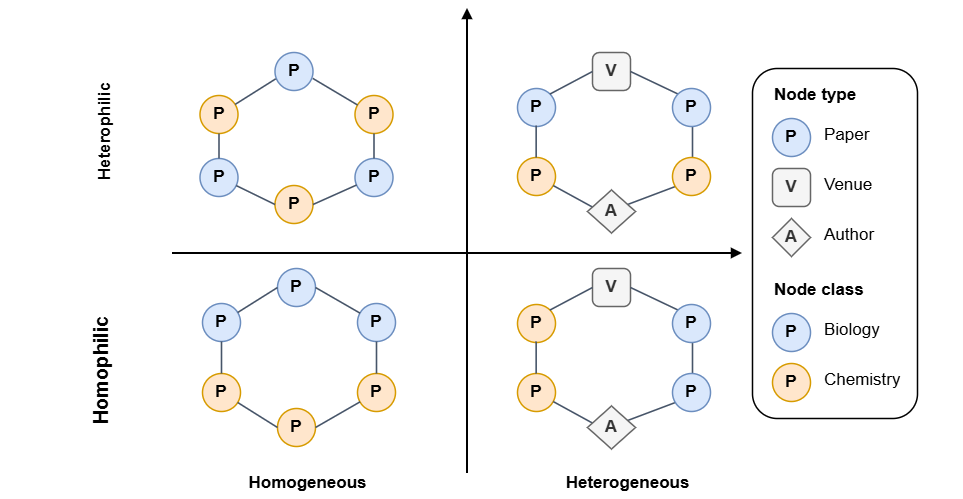
\includegraphics[width=\columnwidth]{figure/Het_HomGraph.drawio.png}
  \caption{An example of heterogeneous heterophilic graph. The graph contains multiple types of nodes and edges, and connected nodes may have different properties.}
  \Description{An example of heterogeneous heterophilic graph. The graph contains multiple types of nodes and edges, and connected nodes may have different properties.}
  \label{fig:het_hom_graph}
\end{figure}

Many existing methods either focus on heterogeneous graph but not consider heterophily \cite{hu2020heterogeneous,mao2023hinormer,he2024spectral,yang2023simple,wang2019heterogeneous,zhang2019heterogeneous} or focus on heterophilic graph but no consider heterogeneous graph \cite{grover2025spectro, yue2025graph,bodnar2022neural,ribeiro2026cooperative}. Recently, several research have targeted heterogeneous heterophilic graphs and captured heterophily by using several approaches, such as using meta-path to construct latent subgraphs suitable for learning heterophily and heterogeneity \cite{lu2026addressing,chen2025adaptive,li2025hetero2net,guo2023homophily,shen2025heterophily,wang2025homophily}, graph rewiring across node types \cite{tao2025cross}, using transformer directly in heterogeneous graphs \cite{lin2025heterophily}, or learnable mappings in heterogeneous graphs \cite{braithwaite2024heterogeneous}. 


